\section{Instruction Set}
\label{ch:is}
The term \emph{reduced} suggests that keeping the Instruction Set (IS) small is a good concept. But
how much can one reduce it? Is there a lower limit? Which are its criteria? There is, of course, no
clear cut measure. An important goal is a certain \emph{completeness}. An IS should make it possible
to compose any more complex operation out of the basic IS. The 2nd goal must be \emph{regularity},
straight rules without exceptions. It facilitates description, understanding, and implementation
enormously.

The principal enemy of regularity and simplicity is the drive for speed, for efficiency. We place
priority on a simple, regular design. Improvements to increase speed can be added at a later stage.
A sound rule to begin is that instructions simple to implement should have priority. Among them are
certainly all logical operations, and because of their frequency the basic arithmetic operations
such as addition and subtraction.

The RISC architecture divides instructions into 3 classes:
\begin{enumerate}
  \item AL instructions operating on registers,
  \item data transfer instructions between registers and memory, and
  \item control (branch) instructions (BI).
\end{enumerate}

\subsection{RI: Register Instruction}
We follow the established convention to provide instructions with 3 register numbers, two specifying
the operands (sources), one the result (destination). Thus we obtain a 3-address computer. It gives
compilers the largest degree of freedom to allocate registers for optimal efficiency. Logical
operations are the conventional AND, OR, XOR. The arithmetic operations are the 4 basic
operations of addition, subtraction, multiplication and division. The inclusion of the latter 2 is to
some degree questionable. They are considered basic in mathematics (although they can be
constructed out of addition or subtraction). Their complexity is indeed of a higher order. This must be
paid by higher “cost”, either in time or circuitry.

Furthermore, we include a set of shift instructions, moving bits horizontally. In fact, a single one,
namely rotation would suffice. Rotation is the best choice because it loses no information, and thus
all other can be constructed out of it. However, we also provide Logical Shift Left (LSL) and
Arithmetic Shift Right (ASR). The former feeds zeroes in at the low end, while the latter replicates
the top bit at the high end. The shift count can be any number between 0 and 31.

All 16 RIs use the same 2 formats:
\begin{enumerate}
  \item F0: both operands are registers;
  \item F1: one operand is a register, the other is a constant held in the instruction itself.
\end{enumerate}

The complete set of RIs is shown in the following codes in an assembler-like form. $R.a$ is
the destination register, and $R.b$ is the 1st operand. The 2nd operand is either register
$R.c$, or the literal ("immediate") $im$. In this case, the \emph{modifier bit} $v$ determines
how the 16-bit constant $im$ is extended into a 32-bit value. The 2 forms of instructions are
encoded as shown in Figure \ref{fig:ri}, $n$ stands for either $R.c$ or $im$.
\begin{verbatim}
   0 MOV a,n   R.a:=n
   1 LSL a,b,n R.a:=R.b  <- n // Logical Shift Left
   2 ASR a,b,n R.a:=R.b  -> n // Arithmetic Shift
      // Right (fill with sign bit instead of zero)
   3 ROR a,b,n R.a:=R.b rot n // ROtate Right

   4 AND a,b,n R.a:=R.b  &  n // logical AND
   5 ANN a,b,n R.a:=R.b  & ~n // ANd Not
   6 IOR a,b,n R.a:=R.b  or n // Inclusive OR
   7 XOR a,b,n R.a:=R.b xor n // eXclusive OR

   8 ADD a,b,n R.a:=R.b  +  n // integeral ADD
   9 SUB a,b,n R.a:=R.b  -  n // SUBstract
  10 MUL a,b,n R.a:=R.b  *  n // MULtiply
  11 DIV a,b,n R.a:=R.b div n // DIVide

  12 FAD a,b,c R.a:=R.b + R.c // Float ADd
  13 FSB a,b,c R.a:=R.b - R.c // Float SuB
  14 FML a,b,c R.a:=R.b * R.c // Float MuL
  15 FDV a,b,c R.a:=R.b / R.c // Float DiV

  v=0 extension of im with 16 zero bits
  v=1 extension of im with 16 one bits
\end{verbatim}
\begin{figure}[h!]
  \centering
  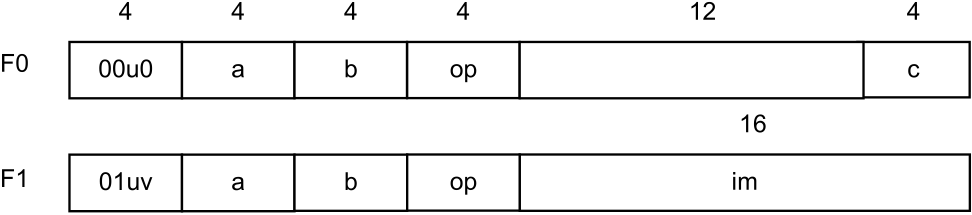
\includegraphics[width=.9\textwidth]{i/2.png}
  \caption{Formats F0 and F1 of RIs}
  \label{fig:ri}
\end{figure}

All RIs (with the exception of multiplication and division) have side effects on the 4 single-bit
condition registers:
\begin{enumerate}
  \item N := bit 31 (the highest bit) of result. Hence, N indicates whether the result is negative.
  \item Z := all bits of result are zero. Z indicates whether the result is zero.
  \item C := carry out bit. (For addition and subtraction only).
  \item V := overflow. (For addition and subtraction only)
\end{enumerate}

These 4 condition registers are tested by BIs. The DIV instruction deposits the remainder in an
auxiliary register H.

RIs contain two modifier bits $u$ and $v$. The instruction MOV with $u$ set to 1 shifts the
immediate value $im$ by 16 bits to the left. Instructions ADD and SUB with the modifier bit $u$ set to 1
add (subtract) the carry bit C, and the MUL instruction with $u$ set to 1 considers the operands as
unsigned numbers, yielding a 64-bit unsigned product.

\subsection{MI: Memory instruction}
There are only 2 MIs, namely \emph{load} and \emph{store}. They specify a destination register
$R.a$ for load, or a source register for store. The address in memory is the sum of register $R.b$ and a
20-bit offset. The format is shown in Figure \ref{fig:mi}.
\begin{figure}[h!]
  \centering
  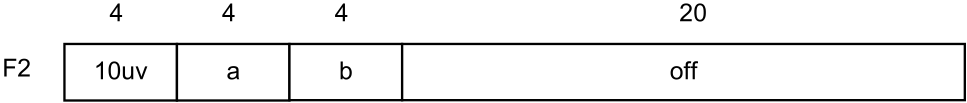
\includegraphics[width=.9\textwidth]{i/3.png}
  \caption{Format F2 of MIs}
  \label{fig:mi}
\end{figure}
\begin{verbatim}
  LD a,b,off // R.a := Mem[R.b+off] u=0 LoaD
  ST a,b,off // Mem[R.b+off] := R.a u=1 STore
\end{verbatim}

The 2nd modifier bit $v$ have the following significance:
\begin{verbatim}
  v=0: word,
  v=1: byte. // implemented on RISC-3 only
\end{verbatim}

\subsection{BI: Branch instruction}
BIs are used to break the sequence of instructions. The next instruction is designated either by
a 24-bit signed offset, or by the value of a register, depending on the modifier bit $u$. It
indicates the length of the jump forward or backward (PC-relative addressing). This offset is
in words, not bytes, as instructions are always a word long.  The modifier $v$ determines
whether the current value of PC be stored in register R15 (the \emph{link} register). This
facility is used for calls to procedures, the value stored is then the return address.
The format is shown in Figure \ref{fig:bi}:
\begin{figure}[h!]
  \centering
  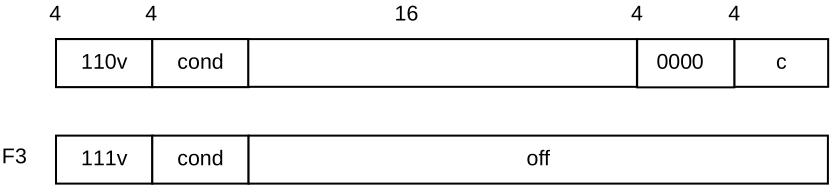
\includegraphics[width=.9\textwidth]{i/4.png}
  \caption{Format F3 of BIs}
  \label{fig:bi}
\end{figure}
\begin{verbatim}
  PC := (u = 1) ? PC + 1 + off : R.c; // u = 0
  IF v = 1 THEN R15 := PC + 1 END;

  B<cond> <dest>; // jump <dest> if <cond> satisfied
\end{verbatim}

The following cond\textcolor{gray}{ition}s are available:
\begin{table}[ht]
  \centering
  \begin{tabular}{l c r|l c l}
    code                     & mean     &                                                   & \textcolor{Plum}{code}                     & mean \\
    ~~~~~cond                & ~~-ing   &                                                   &              ~~~~cond                      & ~~-ing \\\hline
    0000                  MI &$-$Neg.   &                                                N  & \textcolor{Plum}{1}000                  PL & +PLus  & \textcolor{Plum}{\textasciitilde{}}N \\
    0\textcolor{cl1}{001} EQ & $=$Zero  & \textcolor{cl1}{                               Z} & \textcolor{Plum}{1}\textcolor{cl1}{001} NE &$\neq 0$& \textcolor{Plum}{\textasciitilde{}}\textcolor{cl1}{Z} \\
    0\textcolor{cl2}{010} CS & CarrySet & \textcolor{cl2}{                               C} & \textcolor{Plum}{1}\textcolor{cl2}{010} CC & CClear & \textcolor{Plum}{\textasciitilde{}}\textcolor{cl2}{C} \\
    0\textcolor{cl3}{011} VS & oVerflow & \textcolor{cl3}{                               V} & \textcolor{Plum}{1}\textcolor{cl3}{011} VC & VClear & \textcolor{Plum}{\textasciitilde{}}\textcolor{cl3}{V} \\
    0\textcolor{cl4}{100} LS & L.\!|Same& \textcolor{cl4}{            \textasciitilde{}C|Z} & \textcolor{Plum}{1}\textcolor{cl4}{100} HI & HIgh   & \textcolor{Plum}{\textasciitilde{}}(\textcolor{cl4}{\textbullet}) \\
    0\textcolor{cl5}{101} LT & $<$      & \textcolor{cl5}{                        N$\neq$V} & \textcolor{Plum}{1}\textcolor{cl5}{101} GE & $\ge$  & \textcolor{Plum}{\textasciitilde{}}(\textcolor{cl5}{\textbullet}) \\
    0\textcolor{cl6}{110} LE & $\le$    & \textcolor{cl6}{(\textcolor{cl5}{\textbullet})|Z} & \textcolor{Plum}{1}\textcolor{cl6}{110} GT & $>$    & \textcolor{Plum}{\textasciitilde{}}(\textcolor{cl6}{\textbullet}) \\
    0\textcolor{Plum}{111}   & True     & \textcolor{Plum}{                              T} & \textcolor{Plum}{1111}                     & False  & ~~~\textcolor{Plum}{F}
  \end{tabular}
\end{table}
